
% file constrans.tex


\subsection[1D reactive transport]{1D reactive transport with comparison to analytical solution}
\label{l_s_benchmark_1d}

This benchmark describes reactive and conservative mass transport in a one-dimensional aquifer and has two aims. Firstly, a conservative component, a linearly retarded component and a component decaying according to a first order decay are transported and profiles as well as breakthrough curves are compared with the corresponding analytical solution. This comparison is possible only using these simplified reaction types. Secondly, the benchmark is set up in a way that allows to test all element types in this simplified "quasi" one-dimensional setup.

The model aquifer has a length of 100 m in x-direction and 1 m in both y and z direction. Discretization is in element sizes of 1 m in x direction, yielding 100 elements and 101 nodes for the line elements, 100 elements and 202 nodes for the quad elements, 200 elements and 202 nodes for the triangular elements, 100 elements and 404 nodes for the hexahedra elements, 200 elements and 404 nodes for the prism elements and 600 elements and 404 nodes for the tetrahedra elements. To make the boundary conditions consistent with all element types, surfaces in the y-z plane are used to define the boundary conditions at x=0 m and x=100 m.

 The hydraulic conductivity is assumed to be isotropic and constant in the whole aquifer. Flow is from the left to the right (small to large x), induced by fixed head boundary conditions at x=0 and x=100 and a total head difference of 1 m. All components have initial conditions of 0 and a constant concentration boundary condition of 1 at x=0. For the purpose of this benchmark, the concentration units are arbitrary and are therefore normalized. Transport velocity corresponds to 1 m~d$^{-1}$, thus time step length is chosen accordingly as 86400 s (corresponding to 1 d). Total simulation time is 100 d. Thus the Courant number $Co = 1.0$ and the grid Peclet number $Pe_g = 4$, keeping effects of numerical dispersion as well as oscillations sufficiently small.
 All parameters used in this simulation are given in table Tab.~\ref{l_tab_benchmark_1d}.

Three components are used in this benchmark: The component \texttt{ConsTracer} denotes the conservative tracer, for which the advection - dispersion equation is solved. Component \texttt{Decay} is transported according to the advection - dispersion equation with a first order decay rate $\lambda$. Component \texttt{SorbLin} is transported according to the advection - dispersion equation with a linear instantaneous sorption, which corresponds to a retardation of $R = 1 + \frac{1-n}{n} \rho_s K_d = 1 + \frac{0.5}{0.5} \cdot 2000 \cdot0.001 = 3$. All components have the same aqueous phase diffusion coefficient.

%\begin{figure}[htbp]
%\centering
%\includegraphics[width=0.6\textwidth]{figs/fig3_1.eps}
%\caption{Model area and Boundary conditions - adapt to actual setting}
%\label{l_fig_benchmark_1d_1}
%\end{figure}



\begin{table}[htbp]
\caption{Parameters used for benchmark HC$\backslash$1d\_analyt }
\centering
\begin{tabular}{|l|l|l|}
\hline
parameter & value & unit \\
\hline
porosity $\Phi = n $  & 0.5 &  --  \\			
\hline
hydraulic conductivity $K$ & 5.787037$\cdot 10^{-04}$ & ms$^{-1}$ \\
\hline
storage coefficient $S$ & 0.0 & s$^{-1}$ \\
\hline
solid density $\rho_s$ & 2000 &  kg$\cdot m^{-3}$ \\
\hline
density of water $\rho_w$ & 1000 & kg$\cdot m^{-3}$ \\
\hline
viscosity water $\eta$ & 0.001 & Pa$\cdot s$ \\
\hline
dispersion length $\alpha_l$ & 0.25 & m \\
\hline
component diffusion coefficient $D$ & 1.0$\cdot 10^{-9}$ & m$^2$s$^{-1}$ \\
\hline
first order decay rate in water $\lambda$ & 1.0$\cdot 10^{-7}$ & s$^{-1}$ \\
\hline
distribution coefficient $K_d$ & 1.0$\cdot 10^{-3}$ & m$^3$ kg$^{-1}$ \\
\hline
\end{tabular}
\label{l_tab_benchmark_1d}
\end{table}


\subsubsection*{Evaluation method}
Model results are compared to the analytical solution for component profiles along x after a simulation time of 75 days, as well as for breakthrough curves at x=50 m for all components. To facilitate testing of all elements, a batch-file is provided (1D\_all.bat) which reruns the benchmark for all element types by replacing the mesh file accordingly. Results can be viewed using the corresponding layout files by Tecplot. \texttt{companaProfile\_*.lay} is used for displaying the profile results and \texttt{companaBTC\_*.lay} is used for displaying the breakthrough curve results for element type \texttt{*}. The files \texttt{companalytBTC.lpk} and \texttt{companaProfile.lpk} save the simulation results for both types from an earlier GeoSys/RockFlow version for reference.


\subsubsection*{Results}

Results of the simulation and the comparison with the analytical solution are shown in Fig.~\ref{l_fig_benchmark_1d_analyt_1} for the profiles and in Fig.~\ref{l_fig_benchmark_1d_analyt_2} for the breakthrough curves. Numerical results using GeoSys/RockFlow are denoted by symbols, the analytical solution is denoted by the full lines. Correspondence is very good in both cases.

\begin{figure}[htbp]
\centering
\includegraphics[width=0.6\textwidth]{C/figures/1d_analyt_profile.eps}
\caption{Concentration profiles after 100~d}
\label{l_fig_benchmark_1d_analyt_1}
\end{figure}


\begin{figure}[htbp]
\centering
\includegraphics[width=0.6\textwidth]{C/figures/1d_analyt_btc.eps}
\caption{Concentration breakthrough curves at x=50 m }
\label{l_fig_benchmark_1d_analyt_2}
\end{figure}



\begin{table}[htbp]
\centering
\begin{tabular}{|l|l|l|}
\hline
Benchmark & Type & Path \\
\hline
\texttt{1d\_analyt}& HC &  benchmarks$\backslash$C$\backslash$1d\_analyt  \\			
\hline
\end{tabular}
\label{path}
\end{table}


\subsection[2D conservative transport]{2D conservative transport with comparison to analytical solution}
\label{l_s_benchmark_2d}

This benchmark describes the conservative mass transport in a two-dimensional homogeneous aquifer. The main purpose is to compare the numerical results of a conservative mass transport simulation without any reactions with the suitable analytical solution.

The model aquifer has a length of 100 m in the x-direction, 50 m in the y-direction and 1 m in the z direction. The whole domain is discretized into 10560 triangular elements with a constant x and y dimension of 1 m (this value guarantees a Peclet number = 4), except at the boundaries of the injection area where a finer grid is chosen.

The aquifer is assumed to have a homogeneous and isotropic hydraulic conductivity and the constant head boundary conditions on the left (piezometric surface of 2 m) and right side (piezometric surface of 1 m) produce a steady state flow in the right direction. As the material has a constant porosity of 0.5 the resulting flow velocity is 1.1574074 10$^{-3}$ m~s$^{-1}$. Both longitudinal and transversal dispersivity have a value of 0.25, consequently the total simulation time of 80 days is divided into 160 time steps to insure a Courant number lower than 1.
The constant tracer is injected with a relative concentration value of 1.0 from a source 8 m wide set on the left boundary of the aquifer, while the initial concentration of the tracer is zero all over the aquifer domain.

\begin{table}[htbp]
\caption{Parameters used for benchmark HC$\backslash$2d\_analyt }
\centering
\begin{tabular}{|l|l|l|}
\hline
parameter & value & unit \\
\hline
porosity $\Phi = n $  & 0.5 &  --  \\			
\hline
hydraulic conductivity $K$ & 5.787037$\cdot 10^{-05}$ & ms$^{-1}$ \\
\hline
storage coefficient $S$ & 0.0 & s$^{-1}$ \\
\hline
solid density $\rho_s$ & 2000 &  kg$\cdot m^{-3}$ \\
\hline
density of water $\rho_w$ & 1000 & kg$\cdot m^{-3}$ \\
\hline
viscosity water $\eta$ & 0.001 & Pa$\cdot s$ \\
\hline
longitudinal dispersivity $\alpha_l$ & 0.25 & m \\
\hline
transversal dispersivity $\alpha_l$ & 0.25 & m \\
\hline
component diffusion coefficient $D$ & 1.0$\cdot 10^{-9}$ & m$^2$s$^{-1}$ \\
\hline
\end{tabular}
\label{l_tab_benchmark_1d}
\end{table}

\subsubsection*{Evaluation method}

Model results are compared to the Hewson analytical solution (Hewson, Thomas, 1976, Simulation of leachate movement in  the areal plane-A finite element approach: Princeton University, B.S. thesis, 150 p.) for a x-y planar view of the model domain as well as for breakthrough curves at x=60 m and x=80 m after a simulation time of 80 days.
The Hewson solution is more desirable for comparison of this benchmark than the Domenico (1978) solution, because it was developed for a finite width aquifer while the one of Domenico refers to an infinite width aquifer.

\subsubsection*{Results}

Results of the simulation and the comparison with the analytical solution are shown in Fig.~\ref{out60m} for the profiles at 60 m and 80 m, and in Fig.~\ref{tri_ref_layout} for the planar view. Numerical results using GeoSys/RockFlow are represented by the black line, while the Hewson analytical solution is denoted by the red line. Correspondence is very good in both cases and observing the x-y view we can also point out that the numerical simulation is able to properly reproduce lateral and transversal spreading of the constant tracer.

\begin{figure}[htbp]
\centering
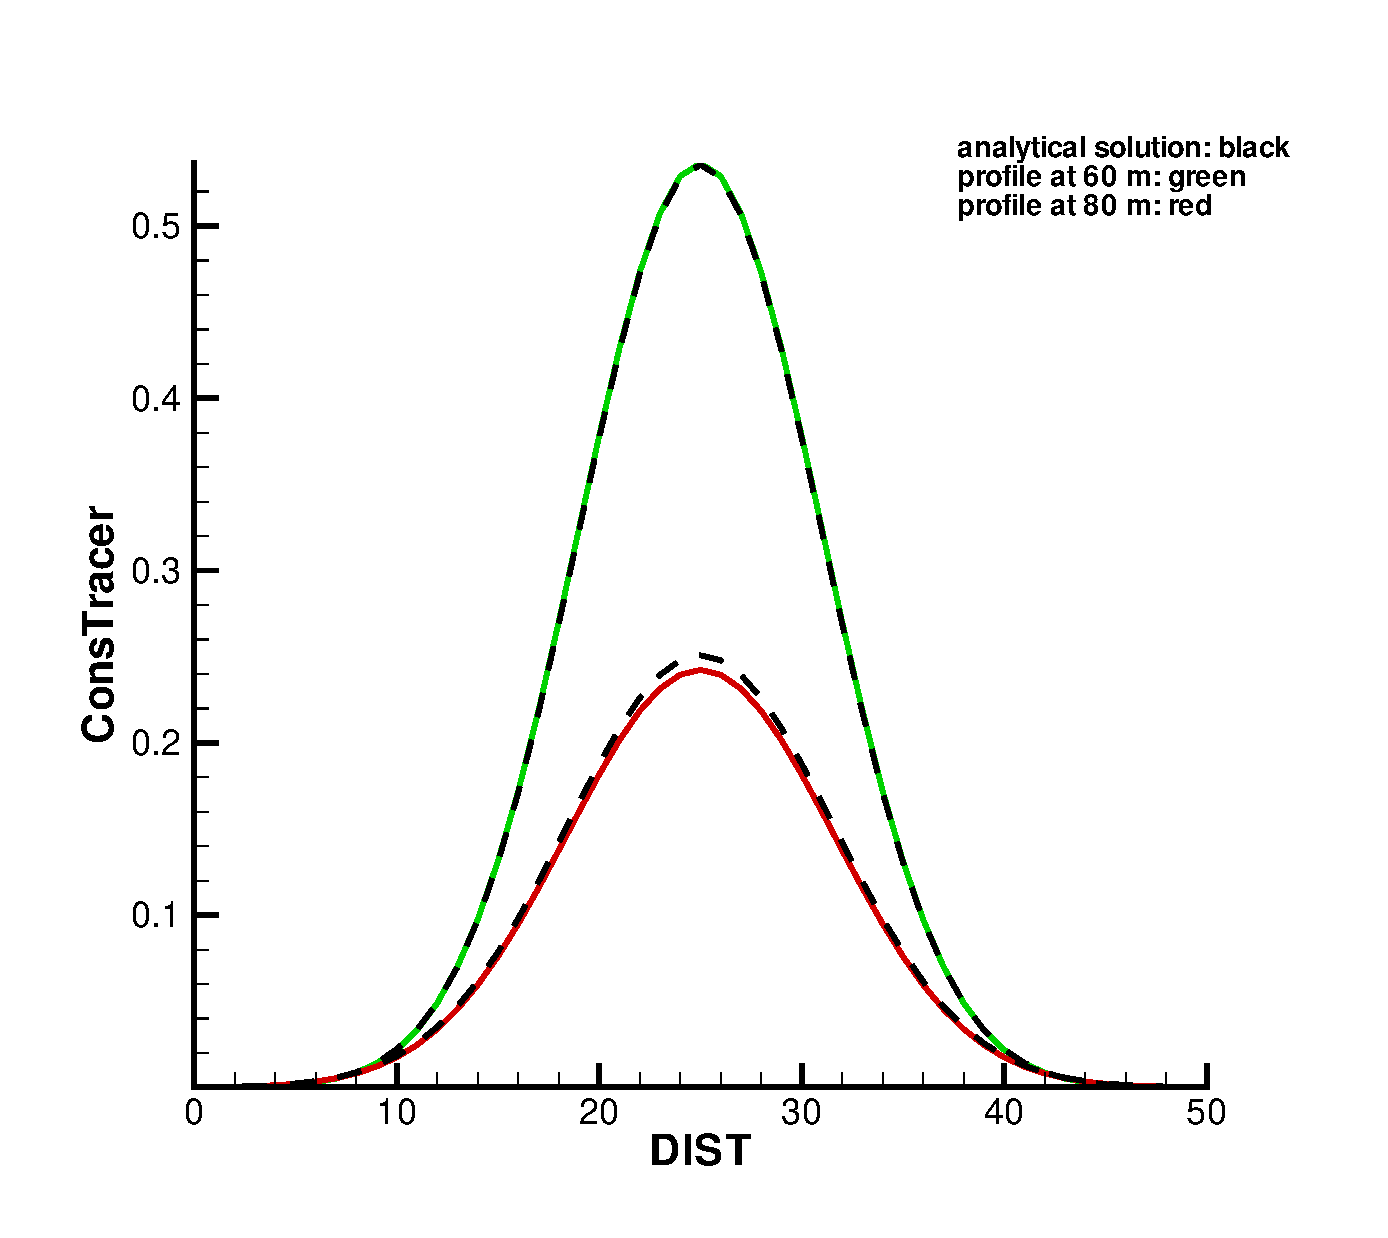
\includegraphics[width=0.6\textwidth]{C/figures/2d_profiles.eps}
\caption{Profiles at 60 m and 80 m after 80~d. Comparison of analytical solution and GeoSys/RockFlow results.}
\label{out60m}
\end{figure}


\begin{figure}[htbp]
\centering
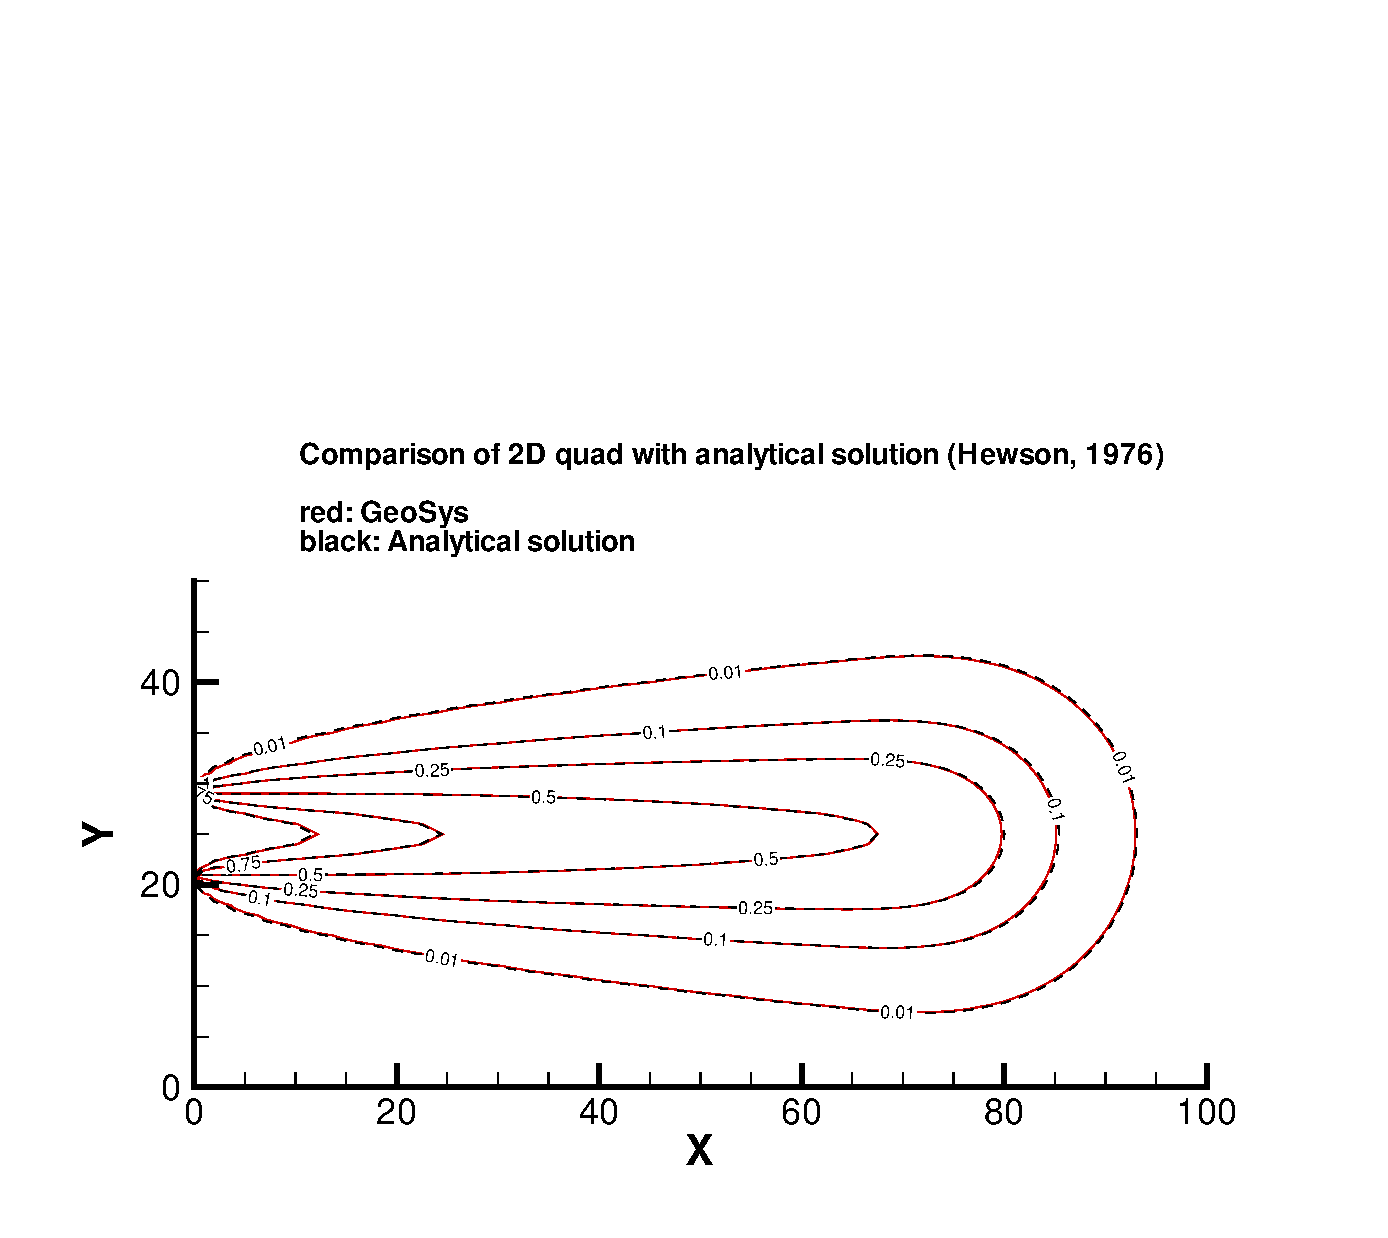
\includegraphics[width=0.9\textwidth]{C/figures/2d_domain.eps}
\caption{Planar x-y view after 80 d. Comparison of analytical solution and GeoSys/RockFlow results.}
\label{tri_ref_layout}
\end{figure}

\begin{table}[htbp]
\centering
\begin{tabular}{|l|l|l|}
\hline
Benchmark & Type & Path \\
\hline
\texttt{2d\_analyt}& HC &  benchmarks$\backslash$C$\backslash$2d\_analyt  \\			
\hline
\end{tabular}
\end{table}





